\documentclass[11pt]{article}
\pdfinfoomitdate=1\pdftrailerid{}
\usepackage[letterpaper,margin=.7in,headheight=15pt,headsep=18pt,footskip=24pt]{geometry}
\usepackage[T1]{fontenc}\usepackage{lmodern,amsmath,amssymb,array,booktabs,fancyhdr,hyperref,tikz}
\renewcommand{\familydefault}{\sfdefault}\setlength{\parindent}{0pt}\setlength{\parskip}{7pt}
\pagestyle{fancy}\fancyhf{}\fancyhead[L]{\small Week 100 / Distance in nested worlds / Facilitator guide}
\fancyfoot[L]{\scriptsize Bellingham Math Circle / Week 100 / W100-FAC-v1}\fancyfoot[R]{\thepage}
\newcommand{\head}[1]{\par\textbf{\large #1}\par}
\newcommand{\sub}[1]{\par\textbf{#1}\par}
\begin{document}
\head{Mathematical overview: distance comes from a hierarchy}
\textbf{The model.} Distinct object cards sit in groups that are nested or disjoint. One outer group contains all cards; each card also has its own singleton group. Positive labels on nonsingleton groups strictly increase outward. The distance of two different cards is the label of their smallest common group; self-distance is zero. Labels are neither group sizes nor physical diameters. Groups may have three or more children.

\textbf{Strong triangle inequality.} The groups that first unite $A,B$ and $B,C$ both contain $B$, so one contains the other. The larger also contains $A,C$. Therefore
\[
d(A,C)\le\max\{d(A,B),d(B,C)\}.
\]
Equivalently, the largest of three pair distances occurs at least twice. Distances $2,4,4$ and $4,4,4$ are possible; $2,2,4$ are not. Equilateral triples must not be excluded by using only binary grouping examples.

\textbf{Balls have many centers and cannot partly overlap.} For $r\ge0$, the radius-$r$ ball about $A$ consists of every card whose distance from $A$ is \emph{at most} $r$, including $A$. If $B$ is in that ball, the strong inequality shows that every member is within $r$ of $B$, and reversing $A,B$ proves the balls are equal. If balls of radii $r\le s$ share a card, use it as center for both: the smaller ball lies in the larger. A supplied radius need not occur as a merger label; a ball can be a singleton.

\textbf{Distances reconstruct the hierarchy.} At each threshold $r$, ``distance at most $r$'' is an equivalence relation: symmetry and reflexivity are immediate, and the strong inequality gives transitivity. Its classes merge as $r$ increases. Complete valid data determine these groups and merger heights, although the drawing's left/right order is arbitrary. An inconsistent triple proves a complete distance table impossible; one altered clue need not identify the original error uniquely.

\textbf{Later number world.} For different integers let $v$ be the number of factors 2 in $a-b$; the 2-adic distance is $2^{-v}$. On cards 0--7 the packet uses eight times that value: 8 for different parity, 4 for equal parity but different remainders modulo 4, and 2 for difference 4. Self-distance is 0. If $2^k$ divides both $a-b$ and $b-c$, it divides their sum $a-c$, proving the strong inequality. Residue groups modulo 2, 4 and 8 make this geometry visible.

\textbf{Discovery, readiness and limits.} Recommended Grades 3--5; the object route requires comparing labels, retaining a new distance rule and coordinating three pair-relations. Adult reading and recording can support a ready younger child, but no K--1 or general Grades 2--3 packet is claimed. The number route additionally needs parity and remainders and can wait for another visit. Experiments motivate the claims; nesting and divisibility prove them. Merger heights are not shortest-road lengths, and this finite example does not construct the completed field of 2-adic numbers.
\newpage
\head{Preparation, shared launch and pacing}
\textbf{Status.} Prepared for organizer review, unpiloted and physically unrehearsed. Actual printing, cutouts, material handling, adult procedures and timing need rehearsal. No younger-table session is implied by the shared demonstration.

\textbf{Per pair.} Six distinct letter-and-shape cards A--F, transparent paper frames or cord loops, labels 2, 4 and 8, removable pair-distance clue cards, and a large workmat. Later use number cards 0--7. Cards around 25 mm and a landscape area about $250\times180$ mm allow visible memberships. Print extra copies of student pages 1, 4, 5 and 7 for cutting cards, preserving the working copies. Keep labels beside frames, and avoid opaque cups that hide cards. Printed small worlds are references; movable materials preserve the child's grouping decisions. Print US Letter single-sided at Actual Size.

\textbf{Staffing.} Two pairs at the middle table if ready and a pair plus rotating checker at the upper table. Rotate builder, clue reader and checker. Three kits and a demonstration board may take about 20 minutes to prepare by hand; this is an estimate. Use the later clue cutouts only after the distance convention is retained. A complete table of distances need not be copied by every child.

\textbf{Launch after handling the frames.} Use unrelated cards X,Y,Z. Put X and Y inside a group labeled 3, then put that group and Z inside a group labeled 6. For X--Z, inspect group 3 (it misses Z), then group 6 (it contains both). Output: distance 6. For X--Y the smallest common group is 3. Slide X within its group: its distances stay unchanged.
\begin{center}
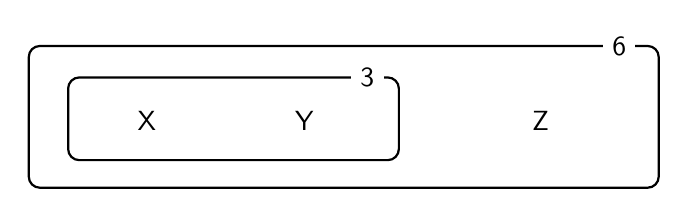
\begin{tikzpicture}[x=1cm,y=1cm]
\draw[rounded corners,thick] (0,0) rectangle(8,1.8);
\node[fill=white] at(7.5,1.8){6};
\draw[rounded corners,thick] (.5,.35) rectangle(4.7,1.4);
\node[fill=white] at(4.3,1.4){3};
\node at(1.5,.85){X};\node at(3.5,.85){Y};\node at(6.5,.85){Z};
\end{tikzpicture}
\end{center}
Before the first ball problem, demonstrate the whole test: center X, radius 3. X is included because its self-distance is 0; Y is included because its distance is 3; Z is excluded because its distance is 6. The output collection is $\{X,Y\}$. A ball is this tested collection, not an arbitrarily drawn oval.

\textbf{A first visit.} Five minutes movement, five minutes handling and launch, 15--20 minutes making and rejecting triples, then 15--20 minutes choosing balls or hidden-world reconstruction. Save clue repair and number geometry for return visits. If an adult continually decides which group is the smallest common one, stay with visible pairs before adding inverse reconstruction. Reading a clue for a child is support; choosing every grouping for them removes the investigation.

\newpage
\head{Visible worlds, contrasting triples and balls}
\sub{Problem 1, page 1: a drawing can move while distances stay fixed}
In the revised visible six-card world, AB first join at 2; D joins AB at 4; C and E join at 2; F joins the other cards only at 8. These are the complete pair distances:
\begin{center}\renewcommand{\arraystretch}{1.2}
\begin{tabular}{c|rrrrrr}
&A&B&C&D&E&F\\\hline
A&0&2&8&4&8&8\\
B&2&0&8&4&8&8\\
C&8&8&0&8&2&8\\
D&4&4&8&0&8&8\\
E&8&8&2&8&0&8\\
F&8&8&8&8&8&0
\end{tabular}\end{center}
Any six pairs can be chosen. Moving cards within their groups, changing frame shapes, rotating the drawing or exchanging left/right placement changes no distances. Moving a card across a group boundary generally does. Check the smallest \emph{common} group: using a group that contains only one chosen card is the characteristic convention error.

\sub{Problem 2, page 2: build or reject six triples}
The possible cases in reading order are $(2,2,2)$, $(2,4,4)$, $(4,4,4)$ and $(2,8,8)$. The impossible cases are $(2,2,4)$ and $(2,4,8)$. Each triple lists AB, AC, BC respectively. For an equilateral case, place the three cards directly inside one group at the common label. For $2,4,4$ put AB together at 2 and add C at 4; for $2,8,8$ add C at 8 instead.

In $2,2,4$, the groups witnessing AB and AC at 2 intersect at A. Nestedness and strict outward increase force them to be the same level-2 group, so BC cannot be 4. In $2,4,8$, the group that unites AC at 4 must also contain B, because AB already join at 2; then BC cannot be 8. These are concrete versions of the strong triangle inequality. Do not turn the common phrase ``isosceles'' into ``exactly two equal sides'': equilateral triangles are allowed.

\sub{Problem 3, page 3: radius tests, including unused radii}
In the revised visible world, radius-3 balls are $\{A,B\}$ about either A or B, $\{C,E\}$ about C, $\{D\}$ about D, and $\{F\}$ about F. The different balls containing B for the listed radii are:
\begin{center}\renewcommand{\arraystretch}{1.25}
\begin{tabular}{c l}
Radii & Collection\\\midrule
0, 1 & $\{B\}$\\
2, 3 & $\{A,B\}$\\
4, 7 & $\{A,B,D\}$\\
8 & $\{A,B,C,D,E,F\}$
\end{tabular}\end{center}
The wording ``balls containing B'' allows centers other than B. It produces the same chain because every member is a center of a ball. A radius need not be a printed group label. Distinct radii can select the same collection; record that collection only once as requested. Radius 0 still contains its center. No card is ever excluded merely because its distance from itself is zero.
\newpage
\head{Hidden geometry and repairing a contradictory clue}
\sub{Problem 4, page 4: reconstruct the five-card world}
The ten clues determine these distance-defined groups: AB at 2, ABC at 4, DE at 2, and all five cards at 8. This differs from the visible six-card world, so the preceding picture does not supply the reconstruction answer. Two drawings may have opposite left/right order or different frame shapes while preserving exactly these groups.

One reconstruction method is to place the closest pairs, then examine how the remaining distances join them. Keep that method in the guide until needed; sorting and choosing a route are part of the student's work. A partner checks all ten cards against the finished drawing. The complete matrix is:
\begin{center}\renewcommand{\arraystretch}{1.2}
\begin{tabular}{c|rrrrr}
&A&B&C&D&E\\\hline
A&0&2&4&8&8\\
B&2&0&4&8&8\\
C&4&4&0&8&8\\
D&8&8&8&0&2\\
E&8&8&8&2&0
\end{tabular}\end{center}
At every threshold, ``distance at most that threshold'' recovers a partition. These partitions determine merger classes, not physical positions. The final question's answer is no. Of the 358 five-card loop structures with labels 2, 4, 8, only AB at 2, ABC at 4, DE at 2 and all five at 8 fits: joining cards whose clue is at most 2 gives AB, DE and C, and at most 4 gives ABC and DE. A second loop around exactly the same cards as another loop (say a 4 around D and E) or a loop around a single card changes no distance; if a child offers one, ask which clue it changes.

\sub{Problem 5, page 5: all one-clue repairs}
After changing AC from 4 to 2, the triple ABC reads AB=2, AC=2, BC=4, which cannot occur. There are exactly three repairs that change one clue to a different allowed value:
\begin{center}\renewcommand{\arraystretch}{1.35}
\begin{tabular}{c p{10.8cm}}
Repair & A world satisfying all ten clues\\\midrule
AC becomes 4 & Restore AB at 2, then C joins at 4.\\
AB becomes 4 & Put AC together at 2, then B joins at 4.\\
BC becomes 2 & Put A, B and C directly in a three-child group at 2.\\\bottomrule
\end{tabular}\end{center}
In every repair, DE remain together at 2, and the ABC group and DE group join at 8. Thus every cross-clue still holds.

\textbf{Completeness.} A change outside AB, AC, BC leaves the contradictory triple unchanged. For AB, the alternatives to 2 are 4 and 8: 4 works, while 8 becomes the unique largest value. The same reasoning applies to AC. For BC, alternatives to 4 are 2 and 8: 2 works and 8 fails. These exhaust all relevant single-clue changes. The original wrong clue cannot be identified from consistency alone; three different repaired worlds fit the allowed changes. Do not imply that restoring AC is the only correction.

\textbf{Hints and readiness.} Offer the ABC clues alone if ten cards overload the group, then return to all the cross-clues. Asking for all repairs is genuine completeness work; pairs may split cases and pool their drawings. If an adult must decide every membership, return to visible pair comparisons before this inverse problem.
\newpage
\head{General explanations, number geometry and the secret-world game}
\sub{Problems 6--7, page 6: beyond a few examples}
Before the general argument, a child can hunt in the Problem 4 world for two balls that partly overlap; every attempt comes out nested or disjoint. Exactly one largest distance is impossible by the nested-group argument in the mathematical overview. To prove the ball facts, let $B$ lie in the radius-$r$ ball around A. For every member X,
\[
d(B,X)\le\max\{d(B,A),d(A,X)\}\le r.
\]
This proves containment in the ball around B; reversing A and B proves equality. If two balls of radii $r\le s$ intersect at Z, use Z as center for both. Every point at distance at most $r$ from Z is also within $s$, proving nesting. The center is the reference card for a distance test, not the middle of a drawn frame. A drawing may suggest these claims, but the argument covers every permitted hierarchy.

\sub{Problems 8--9, page 7: the eight-number world}
Put the even cards $\{0,2,4,6\}$ and odd cards $\{1,3,5,7\}$ into separate groups at 4. Inside them, the residue pairs at 2 are $\{0,4\}$, $\{2,6\}$, $\{1,5\}$ and $\{3,7\}$. The two parity groups join at 8. These four pairs are exactly the radius-3 balls; the even and odd groups are exactly the radius-5 balls. Include the center itself in every ball.

For the elementary three-card explanation, if the cards do not all have the same parity, the two cross-parity distances are both 8. If all have the same parity, three distinct cards cannot all share one remainder modulo 4, because each such class has only two cards in 0--7. Two cards share a remainder and the third differs, giving distances 2,4,4. Thus a largest distance always repeats. This finite number world has no equilateral triple, but general grouped worlds do; do not turn that special feature into a universal restriction.

The divisibility proof in the mathematical overview explains the wider 2-adic connection. On these cards, 0 and 4 are closer than 0 and 1 even though they are farther apart on the ordinary line. The geometry compares agreement in successive remainders, not numerical size. Infinite digit strings and field completion are outside the activity.

\sub{Problem 10, page 8: fewer questions when the answers help}
Asking all $\binom62=15$ unordered pairs always determines the distance table. Some answers permit deductions: if AB=2 and AC=4, then BC must be 4, so that query is unnecessary. If every distance from A to the other five cards is 2, the strong inequality and the smallest allowed positive distance show all pairs are 2. Only five queries were needed in that case.

Fifteen can nevertheless be necessary in the worst case. Suppose every answered query says 8. For any unasked pair, both the all-8 world and a world with just that pair joined at 2 and all other joins at 8 still fit every answer. Therefore one cannot be sure of that pair's value without asking it. The round ends when the builder shows the secret world: any distance in the asker's drawing that differs loses the round, so drawing a pair's value without asking is a risk unless the answers already force it. The game invites economical questioning; this worst-case proof is optional adult depth, not a demand that children optimize every strategy.

\sub{Sources and evidence}
Dovgoshey, \emph{Finite Ultrametric Balls}, \S1, Propositions 1.2 and 1.5, supports the center and nesting properties; Theorem 3.15 discusses finite ball families. The card tasks and elementary proofs here are independently authored. See \texttt{SOURCES.md} for links and distinctions from shortest-road tree geometry and earlier number activities. Exact checks verify every finite case and repair. The QA record covers page inspection and clean source reconstruction. Physical preparation and classroom piloting remain untested; record whether children retain the new distance convention and can make their own grouping choices.

\end{document}
